\documentclass{standalone}
\usepackage{tikz}
\usetikzlibrary{patterns, positioning}


\begin{document}
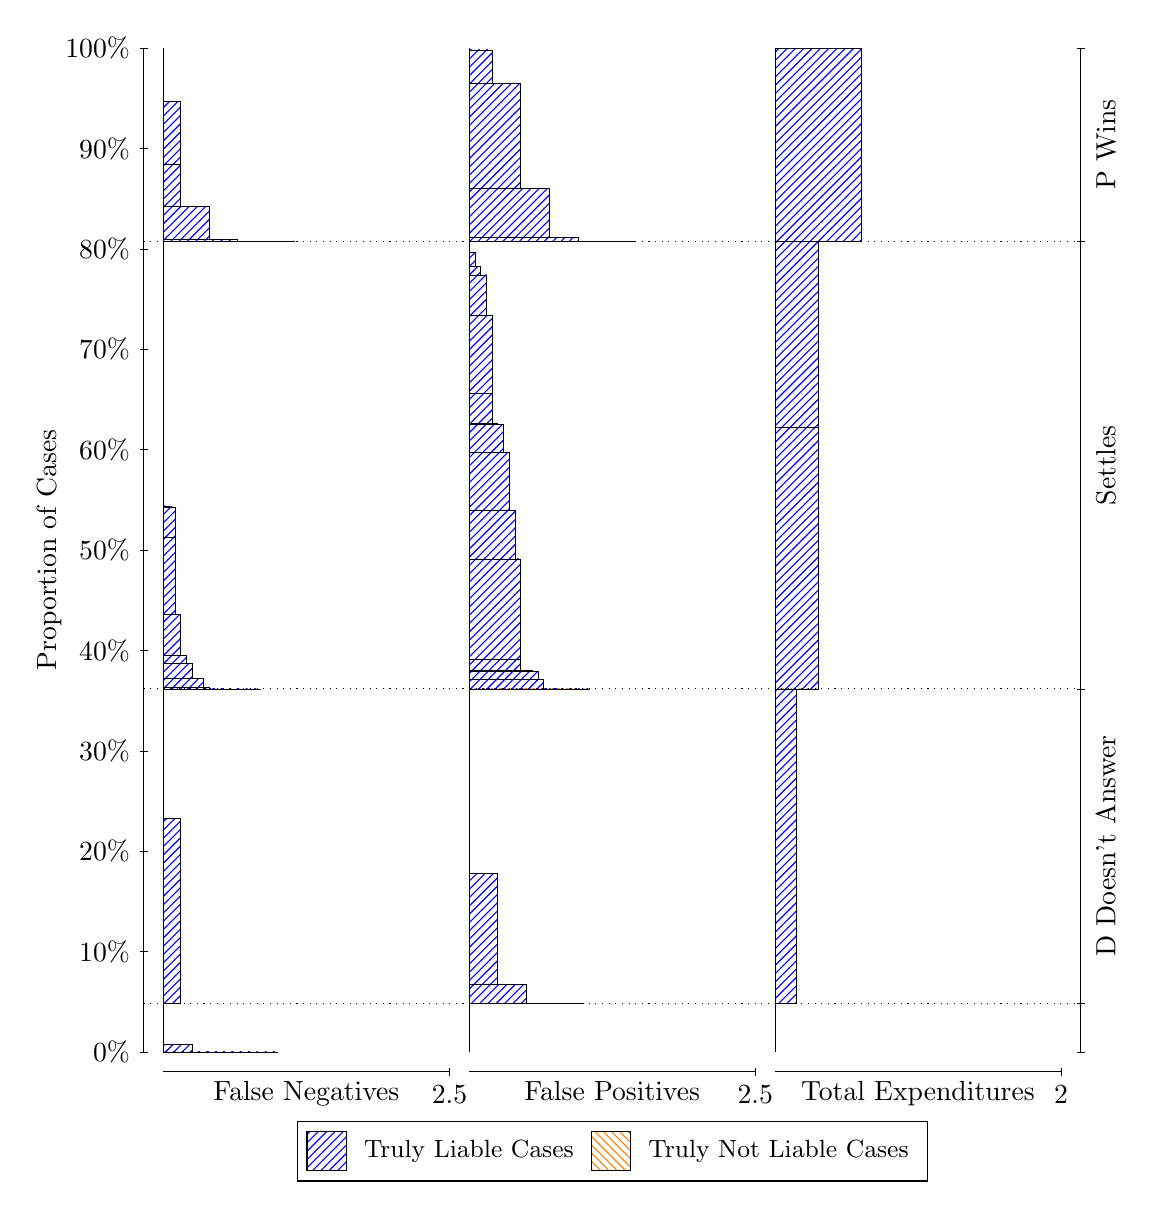
\begin{tikzpicture}
\draw[black, very thin] (1.5,1.75) -- (1.5,14.5);
\node[rotate=90, text=black, anchor=center] at (0.3, 8.125) {Proportion of Cases};
\draw[black, very thin] (1.45,1.75) -- (1.55,1.75);
\node[text=black, anchor=east] at (1.45, 1.75) {0\%};
\draw[black, very thin] (1.45,3.025) -- (1.55,3.025);
\node[text=black, anchor=east] at (1.45, 3.025) {10\%};
\draw[black, very thin] (1.45,4.3) -- (1.55,4.3);
\node[text=black, anchor=east] at (1.45, 4.3) {20\%};
\draw[black, very thin] (1.45,5.575) -- (1.55,5.575);
\node[text=black, anchor=east] at (1.45, 5.575) {30\%};
\draw[black, very thin] (1.45,6.85) -- (1.55,6.85);
\node[text=black, anchor=east] at (1.45, 6.85) {40\%};
\draw[black, very thin] (1.45,8.125) -- (1.55,8.125);
\node[text=black, anchor=east] at (1.45, 8.125) {50\%};
\draw[black, very thin] (1.45,9.4) -- (1.55,9.4);
\node[text=black, anchor=east] at (1.45, 9.4) {60\%};
\draw[black, very thin] (1.45,10.675) -- (1.55,10.675);
\node[text=black, anchor=east] at (1.45, 10.675) {70\%};
\draw[black, very thin] (1.45,11.95) -- (1.55,11.95);
\node[text=black, anchor=east] at (1.45, 11.95) {80\%};
\draw[black, very thin] (1.45,13.225) -- (1.55,13.225);
\node[text=black, anchor=east] at (1.45, 13.225) {90\%};
\draw[black, very thin] (1.45,14.5) -- (1.55,14.5);
\node[text=black, anchor=east] at (1.45, 14.5) {100\%};

\draw[black, very thin] (13.4,1.75) -- (13.4,14.5);
\draw[black, very thin] (13.35,1.75) -- (13.45,1.75);
\node[anchor=west] at (13.35, 1.75) {};
\draw[black, very thin] (13.35,2.3686) -- (13.45,2.3686);
\node[anchor=west] at (13.35, 2.3686) {};
\draw[black, very thin] (13.35,6.3615) -- (13.45,6.3615);
\node[anchor=west] at (13.35, 6.3615) {};
\draw[black, very thin] (13.35,12.044) -- (13.45,12.044);
\node[anchor=west] at (13.35, 12.044) {};
\draw[black, very thin] (13.35,14.5) -- (13.45,14.5);
\node[anchor=west] at (13.35, 14.5) {};

\draw[black, very thin, pattern color=blue, pattern=north east lines] (1.75,1.75) rectangle (3.2033,1.75);
\draw[black, very thin, pattern color=blue, pattern=north east lines] (1.75,1.75) rectangle (2.84,1.75);
\draw[black, very thin, pattern color=blue, pattern=north east lines] (1.75,1.75) rectangle (2.4767,1.7509);
\draw[black, very thin, pattern color=blue, pattern=north east lines] (1.75,1.7509) rectangle (2.1133,1.8513);
\draw[black, very thin, pattern color=orange, pattern=north west lines] (1.75,1.8513) rectangle (1.75,1.8513);
\draw[black, very thin, pattern color=blue, pattern=north east lines] (1.75,1.8513) rectangle (1.75,2.3686);
\draw[black, very thin, pattern color=blue, pattern=north east lines] (1.75,2.3686) rectangle (1.968,4.7135);
\draw[black, very thin, pattern color=orange, pattern=north west lines] (1.75,4.7135) rectangle (1.75,4.7135);
\draw[black, very thin, pattern color=blue, pattern=north east lines] (1.75,4.7135) rectangle (1.75,6.3615);
\draw[black, very thin, pattern color=blue, pattern=north east lines] (1.75,6.3615) rectangle (2.9853,6.3615);
\draw[black, very thin, pattern color=blue, pattern=north east lines] (1.75,6.3615) rectangle (2.6947,6.3615);
\draw[black, very thin, pattern color=blue, pattern=north east lines] (1.75,6.3615) rectangle (2.622,6.3616);
\draw[black, very thin, pattern color=blue, pattern=north east lines] (1.75,6.3616) rectangle (2.5493,6.3616);
\draw[black, very thin, pattern color=blue, pattern=north east lines] (1.75,6.3616) rectangle (2.404,6.3619);
\draw[black, very thin, pattern color=blue, pattern=north east lines] (1.75,6.3619) rectangle (2.3313,6.3781);
\draw[black, very thin, pattern color=blue, pattern=north east lines] (1.75,6.3781) rectangle (2.2587,6.4993);
\draw[black, very thin, pattern color=blue, pattern=north east lines] (1.75,6.4993) rectangle (2.186,6.4998);
\draw[black, very thin, pattern color=blue, pattern=north east lines] (1.75,6.4998) rectangle (2.1133,6.6806);
\draw[black, very thin, pattern color=blue, pattern=north east lines] (1.75,6.6806) rectangle (2.0407,6.7847);
\draw[black, very thin, pattern color=blue, pattern=north east lines] (1.75,6.7847) rectangle (1.968,7.3043);
\draw[black, very thin, pattern color=blue, pattern=north east lines] (1.75,7.3043) rectangle (1.8953,8.2908);
\draw[black, very thin, pattern color=blue, pattern=north east lines] (1.75,8.2908) rectangle (1.8953,8.6716);
\draw[black, very thin, pattern color=blue, pattern=north east lines] (1.75,8.6716) rectangle (1.8227,8.685);
\draw[black, very thin, pattern color=orange, pattern=north west lines] (1.75,8.685) rectangle (1.75,8.685);
\draw[black, very thin, pattern color=blue, pattern=north east lines] (1.75,8.685) rectangle (1.75,12.044);
\draw[black, very thin, pattern color=blue, pattern=north east lines] (1.75,12.044) rectangle (3.4213,12.044);
\draw[black, very thin, pattern color=blue, pattern=north east lines] (1.75,12.044) rectangle (3.058,12.044);
\draw[black, very thin, pattern color=blue, pattern=north east lines] (1.75,12.044) rectangle (2.6947,12.068);
\draw[black, very thin, pattern color=blue, pattern=north east lines] (1.75,12.068) rectangle (2.3313,12.491);
\draw[black, very thin, pattern color=blue, pattern=north east lines] (1.75,12.491) rectangle (1.968,13.029);
\draw[black, very thin, pattern color=blue, pattern=north east lines] (1.75,13.029) rectangle (1.968,13.827);
\draw[black, very thin, pattern color=orange, pattern=north west lines] (1.75,13.827) rectangle (1.75,13.827);
\draw[black, very thin, pattern color=blue, pattern=north east lines] (1.75,13.827) rectangle (1.75,14.5);
\draw[black, very thin, pattern color=orange, pattern=north west lines] (5.6333,1.75) rectangle (5.6333,1.75);
\draw[black, very thin, pattern color=blue, pattern=north east lines] (5.6333,1.75) rectangle (5.6333,2.3686);
\draw[black, very thin, pattern color=orange, pattern=north west lines] (5.6333,2.3686) rectangle (7.0867,2.3686);
\draw[black, very thin, pattern color=blue, pattern=north east lines] (5.6333,2.3686) rectangle (7.0867,2.3686);
\draw[black, very thin, pattern color=blue, pattern=north east lines] (5.6333,2.3686) rectangle (6.7233,2.3705);
\draw[black, very thin, pattern color=blue, pattern=north east lines] (5.6333,2.3705) rectangle (6.36,2.6061);
\draw[black, very thin, pattern color=blue, pattern=north east lines] (5.6333,2.6061) rectangle (5.9967,4.0165);
\draw[black, very thin, pattern color=blue, pattern=north east lines] (5.6333,4.0165) rectangle (5.6333,6.3615);
\draw[black, very thin, pattern color=orange, pattern=north west lines] (5.6333,6.3615) rectangle (7.1593,6.3615);
\draw[black, very thin, pattern color=blue, pattern=north east lines] (5.6333,6.3615) rectangle (7.1593,6.3615);
\draw[black, very thin, pattern color=orange, pattern=north west lines] (5.6333,6.3615) rectangle (7.014,6.3615);
\draw[black, very thin, pattern color=blue, pattern=north east lines] (5.6333,6.3615) rectangle (7.014,6.3615);
\draw[black, very thin, pattern color=orange, pattern=north west lines] (5.6333,6.3615) rectangle (6.8687,6.3615);
\draw[black, very thin, pattern color=blue, pattern=north east lines] (5.6333,6.3615) rectangle (6.8687,6.3617);
\draw[black, very thin, pattern color=blue, pattern=north east lines] (5.6333,6.3617) rectangle (6.796,6.3617);
\draw[black, very thin, pattern color=orange, pattern=north west lines] (5.6333,6.3617) rectangle (6.7233,6.3617);
\draw[black, very thin, pattern color=blue, pattern=north east lines] (5.6333,6.3617) rectangle (6.7233,6.3617);
\draw[black, very thin, pattern color=blue, pattern=north east lines] (5.6333,6.3617) rectangle (6.6507,6.3624);
\draw[black, very thin, pattern color=orange, pattern=north west lines] (5.6333,6.3624) rectangle (6.578,6.3624);
\draw[black, very thin, pattern color=blue, pattern=north east lines] (5.6333,6.3624) rectangle (6.578,6.4837);
\draw[black, very thin, pattern color=blue, pattern=north east lines] (5.6333,6.4837) rectangle (6.5053,6.5841);
\draw[black, very thin, pattern color=blue, pattern=north east lines] (5.6333,6.5841) rectangle (6.4327,6.5969);
\draw[black, very thin, pattern color=blue, pattern=north east lines] (5.6333,6.5969) rectangle (6.36,6.5975);
\draw[black, very thin, pattern color=blue, pattern=north east lines] (5.6333,6.5975) rectangle (6.2873,6.7402);
\draw[black, very thin, pattern color=orange, pattern=north west lines] (5.6333,6.7402) rectangle (6.2873,6.7402);
\draw[black, very thin, pattern color=blue, pattern=north east lines] (5.6333,6.7402) rectangle (6.2873,8.0121);
\draw[black, very thin, pattern color=blue, pattern=north east lines] (5.6333,8.0121) rectangle (6.2147,8.6321);
\draw[black, very thin, pattern color=blue, pattern=north east lines] (5.6333,8.6321) rectangle (6.142,9.3669);
\draw[black, very thin, pattern color=blue, pattern=north east lines] (5.6333,9.3669) rectangle (6.0693,9.7201);
\draw[black, very thin, pattern color=blue, pattern=north east lines] (5.6333,9.7201) rectangle (5.9967,9.7336);
\draw[black, very thin, pattern color=blue, pattern=north east lines] (5.6333,9.7336) rectangle (5.924,10.114);
\draw[black, very thin, pattern color=blue, pattern=north east lines] (5.6333,10.114) rectangle (5.924,11.101);
\draw[black, very thin, pattern color=blue, pattern=north east lines] (5.6333,11.101) rectangle (5.8513,11.62);
\draw[black, very thin, pattern color=blue, pattern=north east lines] (5.6333,11.62) rectangle (5.7787,11.725);
\draw[black, very thin, pattern color=blue, pattern=north east lines] (5.6333,11.725) rectangle (5.706,11.905);
\draw[black, very thin, pattern color=blue, pattern=north east lines] (5.6333,11.905) rectangle (5.6333,12.044);
\draw[black, very thin, pattern color=orange, pattern=north west lines] (5.6333,12.044) rectangle (7.7407,12.044);
\draw[black, very thin, pattern color=blue, pattern=north east lines] (5.6333,12.044) rectangle (7.7407,12.044);
\draw[black, very thin, pattern color=orange, pattern=north west lines] (5.6333,12.044) rectangle (7.3773,12.044);
\draw[black, very thin, pattern color=blue, pattern=north east lines] (5.6333,12.044) rectangle (7.3773,12.044);
\draw[black, very thin, pattern color=orange, pattern=north west lines] (5.6333,12.044) rectangle (7.014,12.044);
\draw[black, very thin, pattern color=blue, pattern=north east lines] (5.6333,12.044) rectangle (7.014,12.098);
\draw[black, very thin, pattern color=orange, pattern=north west lines] (5.6333,12.098) rectangle (6.6507,12.098);
\draw[black, very thin, pattern color=blue, pattern=north east lines] (5.6333,12.098) rectangle (6.6507,12.717);
\draw[black, very thin, pattern color=orange, pattern=north west lines] (5.6333,12.717) rectangle (6.2873,12.717);
\draw[black, very thin, pattern color=blue, pattern=north east lines] (5.6333,12.717) rectangle (6.2873,14.052);
\draw[black, very thin, pattern color=blue, pattern=north east lines] (5.6333,14.052) rectangle (5.924,14.476);
\draw[black, very thin, pattern color=blue, pattern=north east lines] (5.6333,14.476) rectangle (5.6333,14.5);
\draw[black, very thin, pattern color=orange, pattern=north west lines] (9.5167,1.75) rectangle (9.5167,1.75);
\draw[black, very thin, pattern color=blue, pattern=north east lines] (9.5167,1.75) rectangle (9.5167,2.3686);
\draw[black, very thin, pattern color=orange, pattern=north west lines] (9.5167,2.3686) rectangle (9.7892,2.3686);
\draw[black, very thin, pattern color=blue, pattern=north east lines] (9.5167,2.3686) rectangle (9.7892,6.3615);
\draw[black, very thin, pattern color=orange, pattern=north west lines] (9.5167,6.3615) rectangle (10.062,6.3615);
\draw[black, very thin, pattern color=blue, pattern=north east lines] (9.5167,6.3615) rectangle (10.062,9.6839);
\draw[black, very thin, pattern color=orange, pattern=north west lines] (9.5167,9.6839) rectangle (10.062,9.6839);
\draw[black, very thin, pattern color=blue, pattern=north east lines] (9.5167,9.6839) rectangle (10.062,12.044);
\draw[black, very thin, pattern color=orange, pattern=north west lines] (9.5167,12.044) rectangle (10.607,12.044);
\draw[black, very thin, pattern color=blue, pattern=north east lines] (9.5167,12.044) rectangle (10.607,14.5);
\draw[black, dotted] (1.5,2.3686) -- (13.4,2.3686);
\draw[black, dotted] (1.5,6.3615) -- (13.4,6.3615);
\draw[black, dotted] (1.5,12.044) -- (13.4,12.044);
\draw[black, very thin] (1.75,1.5) -- (5.3833,1.5);
\node[text=black, anchor=north] at (3.5667, 1.5) {False Negatives};
\draw[black, very thin] (5.3833,1.45) -- (5.3833,1.55);
\node[text=black, anchor=north] at (5.3833, 1.45) {2.5};

\draw[black, very thin] (5.6333,1.5) -- (9.2667,1.5);
\node[text=black, anchor=north] at (7.45, 1.5) {False Positives};
\draw[black, very thin] (9.2667,1.45) -- (9.2667,1.55);
\node[text=black, anchor=north] at (9.2667, 1.45) {2.5};

\draw[black, very thin] (9.5167,1.5) -- (13.15,1.5);
\node[text=black, anchor=north] at (11.333, 1.5) {Total Expenditures};
\draw[black, very thin] (13.15,1.45) -- (13.15,1.55);
\node[text=black, anchor=north] at (13.15, 1.45) {2};


\node[text=black, centered, rotate=90] at (13.72, 4.365) {D Doesn't Answer};
\node[text=black, centered, rotate=90] at (13.72, 9.2026) {Settles};
\node[text=black, centered, rotate=90] at (13.72, 13.272) {P Wins};

\draw (7.449999999999999,1.5) node[draw=none] (baseCoordinate) {};
\begin{scope}[align=center]
        \matrix[scale=0.5, draw=black, below=0.5cm of baseCoordinate, nodes={draw}, column sep=0.1cm]{
            \node[rectangle, draw, minimum width=0.5cm, minimum height=0.5cm, pattern color=blue, pattern=north east lines] {}; &
            \node[draw=none, font=\small, text=black] (B) {Truly Liable Cases}; &
            \node[rectangle, draw, minimum width=0.5cm, minimum height=0.5cm, pattern color=orange, pattern=north west lines] {}; &
            \node[draw=none, font=\small, text=black] (B) {Truly Not Liable Cases}; \\
            };
\end{scope}

\end{tikzpicture}
\end{document}